% Optimal Control Problems 
\chapter{Optimal Control Problems}

\section{Deterministic Optimal Control} \label{deterministic}


\paragraph{Aim}
To find an optimal temperature trajectory, which minimizes the total volume of fine crystals, represented by the third moment of nucleated crystals ($\mu_{3}^{n}$ ) and maximizes the size of seeded crystals represented by the third moment of seeded crystals ($\mu_{3}^{s}$) in order to satisfy the product quality requirements.

\paragraph{Objective Function}
\begin{equation*}
\max_{T(t)}\lbrace{\mu_{3}^{s}(t_{f}) - \mu_{3}^{n}(t_{f})\rbrace } 
\end{equation*}
For uniformity of shape and size in the crystals in a seeded batch crystallization process, it is essential to ensure that the nucleation phenomena occurs to the minimum and mostly the seeded crystals grow to the desired size at a certain rate, which explains the nature of the objective function .

\paragraph{Active Constraints}
\begin{equation*}
C_{s}\leqslant C \leqslant C_{m}
\end{equation*}
The state variables can be represented as :
\begin{equation*}
y_{i} = \left[\quad C \quad \mu_{0}^{s} \quad \mu_{1}^{s}\quad \mu_{2}^{s}\quad \mu_{3}^{s}\quad \mu_{0}^{n}\quad \mu_{1}^{n}\quad \mu_{2}^{n}\quad \mu_{3}^{n}\quad\right]  
\end{equation*}

Thus, the complete model involving the moment equations consists of nine state equations. 

\subsection{Solution Technique : Steepest Ascent Hamiltonian}

The method involves use of the \textbf{Maximum Principle} discussed by Diwekar et al.\cite{diwekar} in detail. The algorithm of Steepest Ascent utilizes this principle using the Hamiltonian Derivative to move towards the optimum value of Temperature and maximise the objective function. \\
The formulation results in two point boundary value problem, since initial conditions for the state variables and final conditions for the adjoint variables are available. The method also involves introduction of nine additional variables, known as adjoints ($z_{i}$), corresponding to each of the state variable ($y_{i}$), which must satisfy the \textbf{Hamiltonian equation} represented by :
\begin{equation}
H &= \sum_{i = 1}^{9} z_{i}f(y_{i},t,T) 
\end{equation}
The complete problem can be described as :
\begin{align*}
&\max_{T(t)} \lbrace{ y_{5}(t_{f}) - y_{9}(t_{f})}\rbrace \\
&\frac{dy_{i}}{dt} = f(y_{i},t,T) \\
&\frac{dz_{i}}{dt} = \sum_{j=1}^{9} z_{j}\frac{\partial f(y_{i},t,T)}{\partial y_{i}} = f(y_{i},z_{i},t,T) \\
\end{align*}
with the following initial conditions:\\
$t_{0} = 0$ and $t_{f} = 1800s$ (batch time)
\begin{align*}
&y_{i}(t_{0}) = \left[ 0.1743 \quad 66.66 \quad 1.83\times10^{4}\quad 5.05\times10^{6} \quad 1.93\times10^{9} \quad 0.867 \quad 0 \quad 0 \quad 0 \right] \\
&z_{i}(t_{f}) = \left[  0 \quad 0 \quad 0 \quad 0 \quad 1 \quad 0 \quad 0 \quad 0 \quad -1 \right] 
\end{align*}
\paragraph{Algorithm}
\begin{enumerate}
\item An initial temperature $T(t) = 323 K$ is assumed for the entire time horizon.
\item The differential equations for state variables are integrated using the initial conditions for a time step of 1s .
\item The value of the adjoint variables are computed by backward integration for the same time step used in the previous.
\item For evaluation of the Hamiltonian derivative, an analytical method proposed by Benavides and Diwekar\cite{benavides},  is used in which we an additional variable corresponding to each of the state and adjoint variable is introduced.
\item The variable $\theta_{i}$ corresponds to each of the state variable $y_{i}$ and the variable $\phi_{i}$ corresponds to each of the adjoint variable $z_{i}$, respectively.
\item The Hamiltonian derivative is now calculated at each time step  as :
\begin{align}
&\theta = \frac{dy_{i}}{dT} \quad and \quad \phi_{i} = \frac{dz_{i}}{dT} \\
&\frac{dH}{dT} = \sum_{i=1}^{9} \left( \frac{dH}{dy_{i}}\right)\left(	\frac{dy_{i}}{dT} \right) + \sum_{i=1}^{9} \left(\frac{dH}{dz_{i}}\right)\left(\frac{dz_{i}}{dT} \right)
\end{align}
\item The  convergence criterion $(\frac{dH}{dT}<$ tolerance) is verified. If it is not satisfied, the temperature $T(t)$ is updated using this gradient\cite{yenkie}.
\begin{equation}
T^{new}(t) = T^{old}(t) + M\left(\frac{dH}{dT} \right)
\end{equation}
\item The concentration is evaluated  at that time step and compared with first with the saturation concentration ($C_{s}$) and the metastable concentration($C_{m}$) to validate the active constraints.
\item Iterations of above steps are repeated.
\end{enumerate}


\subsection{Results}

The following fixed kinetic parameters were used in the deterministic modelling. 

\begin{center}
\begin{table}[!h]
\centering
\begin{tabular}{|c|c|}
\hline
Parameters & Experimental Values \\
\hline
\multicolumn{2}{|c|}{Growth Kinetics} \\
\hline
$k_{g}$ & $1.44\times10^{8} \mu m s^{-1}$ \\
$E_{g}/R$ & $4859K$ \\
$g$ & $1.5$ \\
\hline
\multicolumn{2}{|c|}{Nucleation Kinetics} \\
\hline
$k_{b}$ & $285 (s \mu m^{3})^{-1}$ \\ 
$E_{b}/R$ & $7517K$ \\
$b$ & $1.45$ \\
\hline
\end{tabular}
\caption{Parameter Values for Batch Crystallizer$^{5-7}$}
\label{Table1}
\end{table}
\end{center}

\begin{itemize}
\item The model was implemented both using \textbf{Python} and \textbf{Matlab} producing similar results. 
\item Matlab employed use of \textbf{ode15s} for performing the forward and backward integrations which is used to solve stiff-differential equation. 
%In Python it was performed through \textbf{Explicit Euler} method.
\item A tolerance value of $10^{-2}$ is used for computation of the Hamiltonian Derivative profile. The value of M was selected suitably after experimentation. 
\end{itemize}
The following results were obtained: \\
\begin{figure}[h!] 
\caption{Objective Function ($\mu_{3}^{s}(t) - \mu_{3}^{n}(t)$)}
\begin{center}
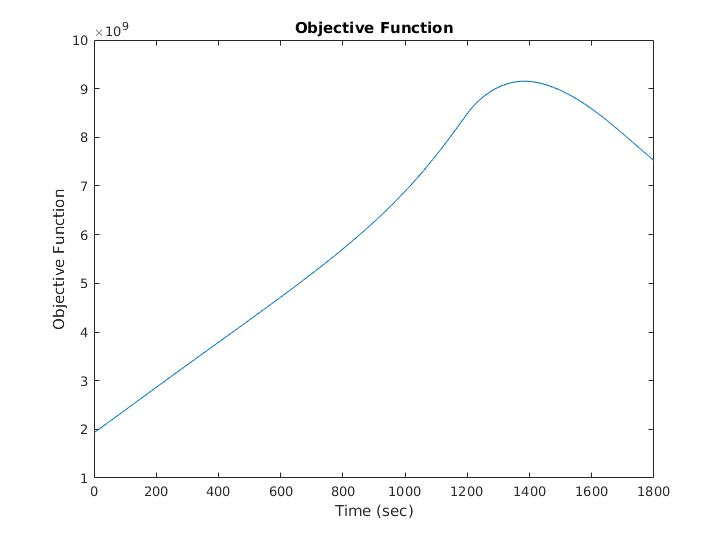
\includegraphics[width=4in]{objective.jpg}
\end{center}
\end{figure}
\begin{figure}[h!] 
\caption{Depicts the cooling profile for the controlled variable T(t) obtained at the final iteration}
\begin{center}
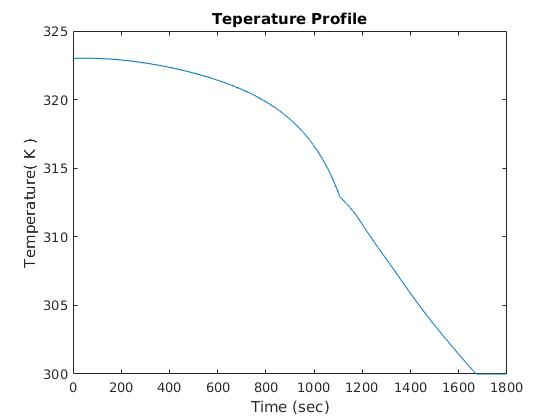
\includegraphics[width=4in]{temp.jpg}
\end{center}
\end{figure}
\clearpage
The change of the Hamiltonian Derivative($\frac{dH}{dT}$) after each iteration is shown below : 
\begin{figure}[h!]
  \centering
  \begin{minipage}[b]{0.4\textwidth}
    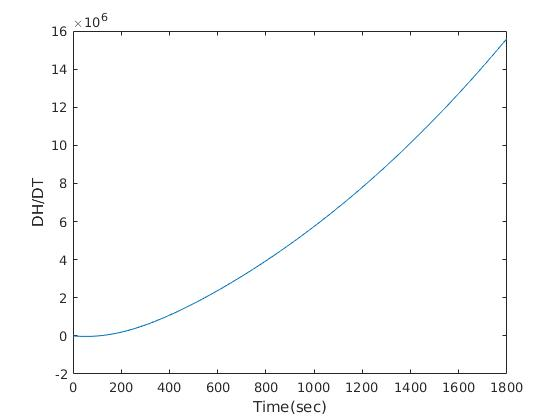
\includegraphics[width=\textwidth]{h1.jpg}
    \caption{Iteration 1}
  \end{minipage}
  \hfill
  \begin{minipage}[b]{0.4\textwidth}
    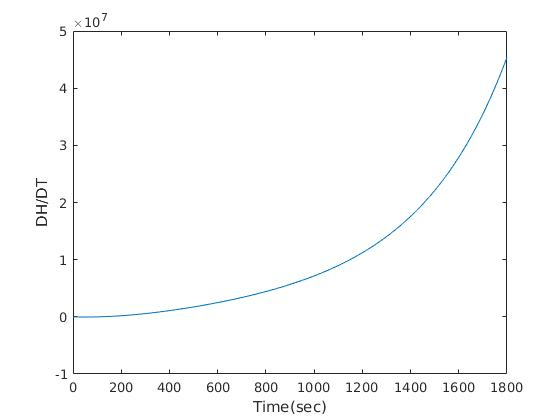
\includegraphics[width=\textwidth]{h2.jpg}
    \caption{Iteration 2}
  \end{minipage}
\end{figure}
\begin{figure}[h!]
  \centering
  \begin{minipage}[b]{0.4\textwidth}
    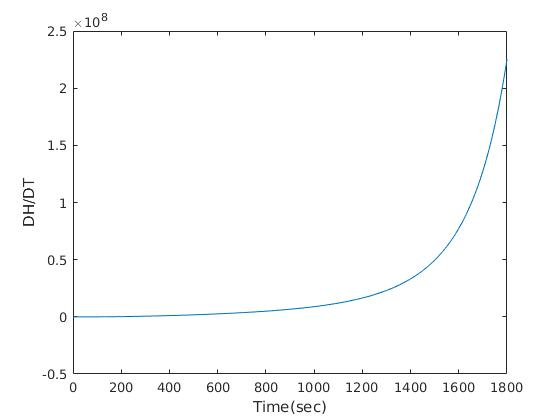
\includegraphics[width=\textwidth]{h3.jpg}
    \caption{Iteration 3}
  \end{minipage}
  \hfill
  \begin{minipage}[b]{0.4\textwidth}
    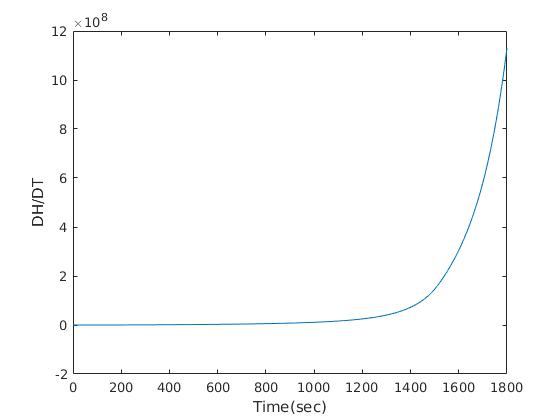
\includegraphics[width=\textwidth]{h4.jpg}
    \caption{Iteration 4}
  \end{minipage}
\end{figure}
\begin{figure}[h!]
  \centering
  \begin{minipage}[b]{0.4\textwidth}
    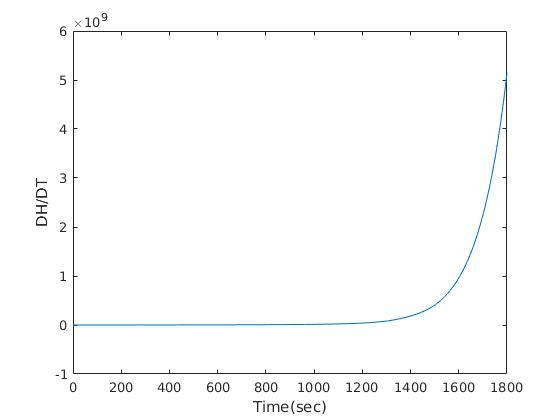
\includegraphics[width=\textwidth]{h5.jpg}
    \caption{Iteration 5}
  \end{minipage}
  \hfill
  \begin{minipage}[b]{0.4\textwidth}
    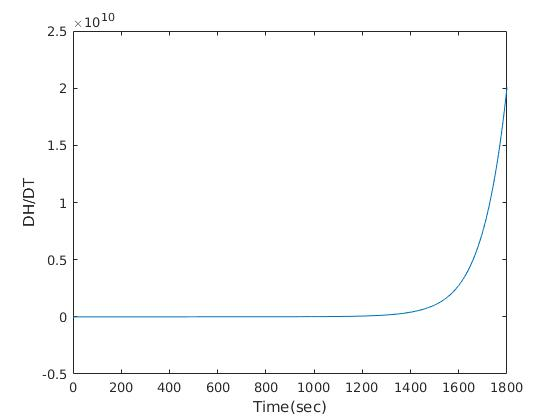
\includegraphics[width=\textwidth]{h6.jpg}
    \caption{Iteration 6}
  \end{minipage}
\end{figure}